%==================================================================%
% Author : Pando Muñoz, Manuel                                     %
%          Sánchez Barreiro, Pablo                                 %
% Version: 1.0, 30/03/2011                                         %
%                                                                  %
% Memoria del Proyecto Fin de Carrera                              %
% Archivo raíz para el capítulo de descripción general             %
%==================================================================%


\chapterheader{Descripción y Planificación}{Descripción y Planificación del Proyecto}
\label{chap:planificacion}


El presente cap\'itulo describe en líneas generales el ámbito funcional del proyecto, para delimitar su alcance, la metodología a usar durante el desarrollo del sistema y los requisitos de alto nivel del mismo, extraídos del ámbito funcional descrito.

\chaptertoc

\section{Descripción Funcional del Sistema}
\label{sec:planificacion:descFuncional}

En la siguiente sección se describe el ámbito funcional del sistema software que deseamos construir, es decir, del \emph{DrManhattan}, que es un \emph{Sistema de Control de Accesos a Red para los Laboratorios de la Facultad de Ciencias}.\newline

%==========================================================================%
% NOTA(Pablo): Esta información se considera sabida, por lo que no hay
%              que aportarla
%==========================================================================%
% Definirlas de modo correcto es muy importante, ya que los requisitos de
% alto nivel dependen directamente y si estos son incorrectos, obtendríamos
% una aplicación inútil que no cumple con lo requerido. \newline

El objetivo del \emph{DrManhattan} es controlar el acceso a la red local, existente en cada laboratorio de la Facultad de Ciencias de la Universidad de Cantabria, de los computadores conectados a ella.
%==========================================================================%
% NOTA(Pablo): Ya sabemos que es lo que hay que controlar, ahora un buen
%              Ingeniero de Requisitos debe averiguar por qué hay que
%              controlarlo y para qué hay que controlarlo. Esos son los
%              dos objetivos principales y justificación última de cada
%              decisión que se tome en el proyecto
%
%              El por qué y el para qué te lo he escrito yo
%==========================================================================%
Se desea realizar dicho control sobre todo durante la realización de pruebas evaluables, de cara a evitar que se realicen accesos a contenidos no autorizados (e.g., páginas de internet con posibles soluciones a los problemas planteados, el directorio de trabajo de algún compañero, etc.) durante la realización de dichas pruebas. El sistema que se venía utilizando hasta ahora para evitar el mal uso de la red local consistía simplemente en desconectar la alimentación del concentrador de interconexión, deshabilitando la red. Es decir, se aplicaba el principio de muerto el perro, se acabó la rabia.
\newline

No obstante, el tener los diversos computadores interconectados mediante una red local, no sólo tiene inconvenientes, sino que también posee varias ventajas. Por ejemplo, ayuda a facilitar la distribución de material electrónico que resulte necesario para la realización del examen. También puede ser de gran utilidad para recoger los ejercicios realizados por los alumnos de una manera rápida y cómoda, ya que el alumno sólo tendría que enviar el material producido durante la prueba al computador o dirección que le indique el profesor. El método utilizado actualmente para realizar esta tarea consiste en que el profesor acude al computador del alumno cuando este desea entregar los ejercicios realizados y copia tales ejercicios en una memoria USB. Este proceso es lento, tedioso y en muchas ocasiones las memorias USB no son reconocidas por los computadores del laboratorio, lo que exige recurrir a otras técnicas. El tiempo empleado por los docentes para recopilar los ejercicios realizados por los alumnas suele oscilar entre la media hora y la hora completa, mientras que usando la red local dicho proceso podría realizarse en cuestión de minutos (cuando no menos).
\newline

%==========================================================================%
% NOTA(Pablo): Como ahora tenemos un por qué y un para qué, el siguiente
%              párrafo sale por si sólo como consecuencia de lo anterior
%              Sale el concepto de ordenador distinguido, por lo que es
%              mejor darle nombre
%==========================================================================%

Por tanto, el acceso de los computadores a la red local (e internet), se deberá controlar desde un computador distinguido, al que llamaremos \emph{Watchman},
que será normalmente el computador asignado al docente. Dicho computador será el encargado de conceder y denegar el acceso a la red al resto de computadores conectados a la red local.
\newline

Se desea que el acceso a la red esté habilitado en las siguientes circunstancias:
\begin{enumerate}
	\item Al comienzo de la realización de las pruebas, de forma que el docente pueda distribuir material electrónico necesario o de interés para la realización de la prueba (e.g., manuales, el enunciado de la prueba, etc.) entre los diferentes computadores de forma cómoda y eficiente.
	\item Cuando el alumno haya finalizado la prueba, de forma que se puedan enviar los resultados a través de la red, evitando el tedioso proceso de tener que recogerlos de forma individual mediante copia en un memoria USB o dispositivo similar. En estos casos, sería además deseable, con objeto de evitar posteriores problemas, que el sistema comprobase la integridad de los archivos recibidos, es decir, que comprobase que no se han sufrido alteración alguna durante la transmisión.
\end{enumerate}

Durante el periodo de tiempo que un alumno esté realizando una prueba, se debe denegar el acceso a la red del computador que esté utilizando para la realización de la prueba.
\newline

%==========================================================================%
% NOTA(Pablo): Ya tienes la información sobre cuando se conectan y
%              desconectan los computadores a la red
%==========================================================================%

Por tanto, la secuencia de realización de una prueba evaluable sería tal como sigue:

\begin{enumerate}
	\item El profesor y los alumnos acceden al aula y encienden sus correspondientes computadores. El acceso a la red está habilitado para todo el mundo.
	\item El profesor envía el material necesario para la realización de la prueba a los computadores de los alumnos.
	\item A continuación, una vez que un alumno comienza la prueba, se le deniega el acceso a la red al computador que esté utilizando. %El inicio de la prueba lo puede señalar tanto el alumno individualmente desde su propio computador como el profesor desde el computador que actué como \emph{Watchman} de forma simultánea para todos los alumnos.

%==============================================================================%
% NOTA(Manuel): Yo entendía que era el profesor el único que indicaba el inicio
%               de la prueba, de modo que empiecen todos los alumnos a la vez.
%==============================================================================%


	\item Si durante la realización de la prueba un alumno considera que ha acabado y está satisfecho con los resultados producidos, indicará al sistema que ha concluido la prueba. Los ficheros producidos como material evaluable se enviarán al \emph{Watchman}. Se comprobará que se han recibido correctamente y no están corruptos, por lo que se pueden abrir y leer sin problema alguno. Obviamente, para el envío de los ficheros de resultados habrá que habilitar de nuevo la red, pero se ha de evitar que el alumno pueda modificar dichos ficheros.
	\item Debe existir también la posibilidad de que el docente decida que el tiempo de realización de la prueba ha concluido, por lo que deberá realizarse todo el proceso descrito en el punto anterior, pero para todos los computadores que se encuentren activos en ese momento y siendo el proceso iniciado desde el \emph{Watchman}, en lugar de desde el propio computador del alumno.
\end{enumerate}


%==========================================================================%
% NOTA(Pablo): El sistema ya está descrito, vamos ahora con los aspectos
%              adicionales
%==========================================================================%
Además, se guardarán registros de los eventos ocurridos en cada prueba, con el objetivo de tener información que permita auditar el transcurso de la misma. Dicho registro debe mantener constancia de eventos tales como hora de inicio de la prueba, hora de entrega de cada ejercicio, número de ficheros que se entregan, etc.
\newline

Para comodidad del alumno, en las pruebas con hora de finalización predeterminada se mostrará en la interfaz de la aplicación los minutos restantes hasta el final.
\newline

%==========================================================================%
% NOTA(Pablo): Observa el párrafo de enlace
%==========================================================================%

La siguiente sección detalla la metodología de desarrollo que usaremos para la construcción de este sistema.

\section{Metodología de Desarrollo}
\label{sec:planificacion:metodologia}

En esta sección se describe la metodología utilizada para desarrollar el sistema.
\newline

Se ha escogido el proceso de desarrollo \emph{iterativo e incremental} que suele ser parte esencial en las metodologías de desarrollo ágiles\cite{AGIL:2003}.
\newline

%Qué es
La idea principal de este proceso se basa, como su nombre, en iteraciones e incrementos, que no son lo mismo.
El software se construye mediante tareas repetitivas, \emph{iteraciones}, en las que se añaden nuevas funcionalidades progresivamente, \emph{incrementos}, para crear una versión del sistema que cumple más requisitos que la anterior. Se realizan tantas iteraciones sean necesarias hasta que todos los requisitos se hayan implementado y, por tanto, el sistema este finalizado.
\newline


\begin{figure}
    \centering
    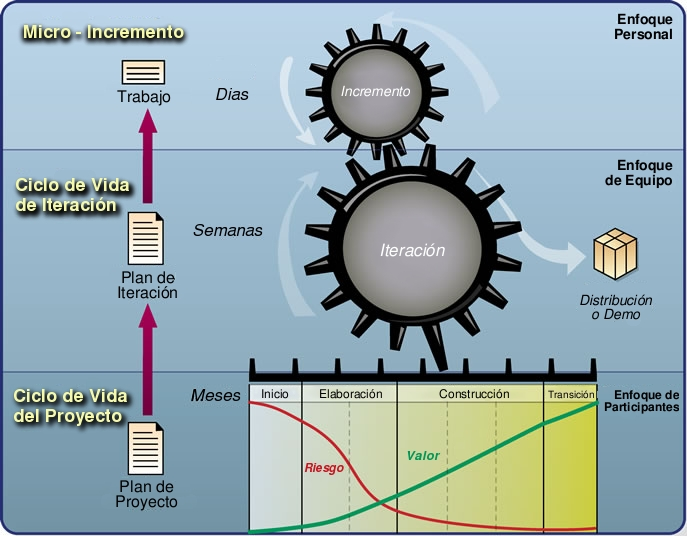
\includegraphics[width=\linewidth]{planificacion/iteracionIncremento}
    \caption{Diferencia entre iteración e incremento.\cite{UP:2006}}
    \label{fig:planificacion:iteracionIncremento}
\end{figure}

Es decir, una iteración es un mini-proyecto en el que se obtiene una versión de cada una de las piezas del sistema, sean código o no, y un incremento se puede medir como la diferencia entre una iteración y la anterior.
\newline

El proceso se divide en cuatro partes fundamentales:

\begin{enumerate}

	\item \textbf{Iniciación:} en esta fase se describe el ámbito funcional del sistema, los requisitos de alto nivel y se identifican posibles riesgos. Hay que comprender el sistema y sus límites.

	\item \textbf{Elaboración:} el objetivo principal de esta fase es el de crear la arquitectura básica, para tener una visión de cómo será el sistema completo y además, proponer soluciones a los riesgos identificados.

	\item \textbf{Construcción:} cómo su nombre indica, esta es la fase dónde se construye y prueba la aplicación. Se realiza un pequeño proceso en cascada en cada iteración de esta fase.

	\item \textbf{Transición:} se despliega el sistema y finaliza el proceso.

\end{enumerate}


\begin{figure}[!h]
    \centering
    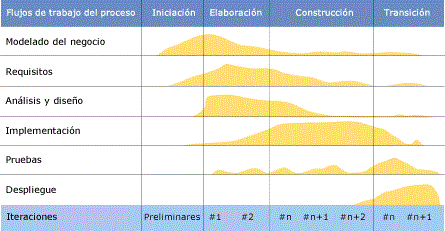
\includegraphics[]{planificacion/trabajoFases}
    \caption{Carga de trabajo en las diferentes fases.\cite{RUP:2003}}
    \label{fig:planificacion:trabajoFases}
\end{figure}

Cada una de estas fases, como es lógico, puede tener más de una iteración, en función del tamaño del proyecto, con tareas propias de la etapa en que se esté, así por ejemplo, en la etapa de construcción, en cada iteración se escoge un grupo de requisitos de alto nivel, se refinan, y partiendo de la versión del sistema obtenida en la iteración anterior, se diseñan, implementan y prueban esos requisitos, creando la versión que se utilizará en la siguiente iteración. En la figura \ref{fig:planificacion:trabajoFases} se muestra una aproximación de lo que sería la carga de trabajo que requieren las distintas tareas en función de la etapa en que se encuentre el proyecto.
\newline

Al finalizar el proceso obtenemos tanto el código de la aplicación, como modelos y documentación de la misma que se van creando a lo largo de las iteraciones.
\newline


Las principales razones por las que se ha escogido este tipo de proceso y no otro son:

\begin{itemize}

	\item[\ding{70}] Poca incertidumbre a la hora de diseñar y planificar, ya que al realizarse en cada iteración y no del sistema completo, se tiene mayor comprensión de los riesgos y de las tareas a realizar.

	\item[\ding{70}] Se adapta bien a cambios de requisitos.

	\item[\ding{70}] Si se priorizan los requisitos para implementarlos en las primeras iteraciones de la construcción, se obtiene una aplicación con funcionalidades clave en la que el cliente puede decidir si está o no correcto.

	\item[\ding{70}] Al trabajar con un subconjunto de requisitos en cada iteración la complejidad se reduce, lo que facilita que se reduzca también el número de errores producidos.

\end{itemize}



De la primera fase, \emph{iniciación}, la descripción funcional detallando el alcance del sistema está descrita en la sección \ref{sec:planificacion:descFuncional}, a continuación se muestra un diagrama de casos de uso, basado en esa descripción y en la siguiente sección se describen los requisitos de alto nivel extraídos.

\begin{figure}[!h]
    \centering
    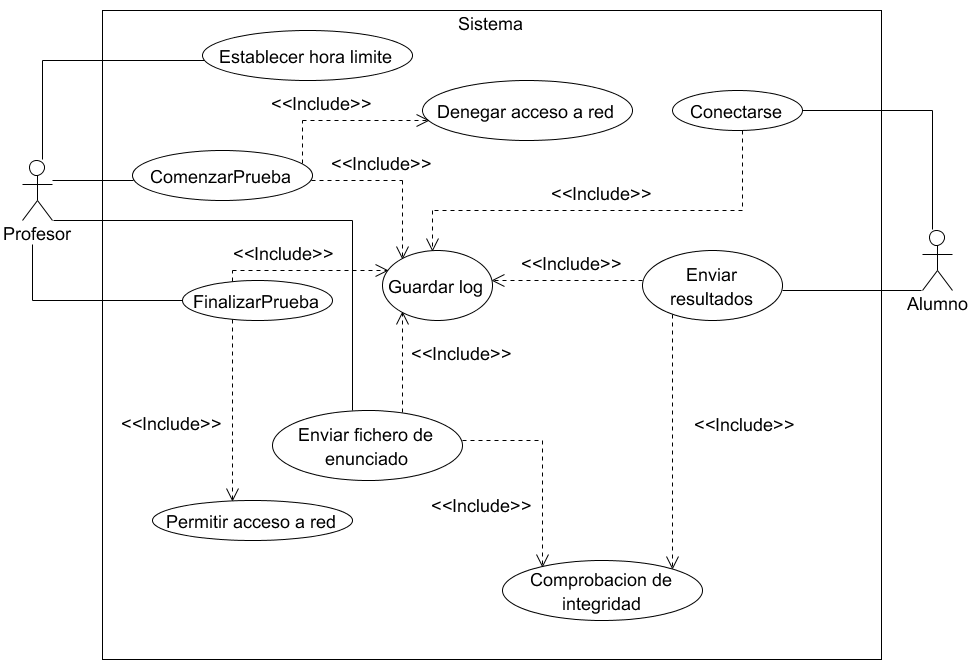
\includegraphics[width=\linewidth]{planificacion/casosUsoSistema2}%[width=.90\linewidth]{planificacion/casosUsoSistema}
    \caption{Diagrama de casos de uso del sistema}
    \label{fig:planificacion:casosUso}
\end{figure}



\section{Requisitos de Alto Nivel del Sistema}
\label{sec:planificacion:requisitos}

%==========================================================================%
% NOTA(Pablo): Ligando las secciones, que siempre queda muy bien
%==========================================================================%
Esta sección describe el segundo paso en nuestro proceso de desarrollo, de acuerdo a la metodología descrita en la sección anterior, que es la identificación de los requisitos de alto nivel que ha de satisfacer nuestro sistema software, de acuerdo a la descripción del ámbito funcional proporcionada en la Sección~ \ref{sec:planificacion:descFuncional}.
\newline
%==========================================================================%
% NOTA(Pablo): Todo esto se considera sabido, por lo que no hay que
%              escribirlo
%==========================================================================%
% Definirlas de modo correcto es muy importante, ya que los requisitos de
% alto nivel dependen directamente y si estos son incorrectos, obtendríamos
% una aplicación inútil que no cumple con lo requerido.
%
% Un requisito es una propiedad que debe ser exhibida por un software para
% resolver un problema particular.
% Los requisitos han de tener ciertas características, entre ellas ser:
% \begin{itemize}
%    \item \emph{No ambiguos,} no puede haber varias interpretaciones para un %requisito puesto que se puede optar por una solución no deseada por el cliente.
%
%\item \emph{Entendible,} se comprende fácilmente el significado.
%
%\item \emph{Verificable,} es necesario que existan técnicas para comprobar que cada requisito es construido correctamente.
%
%\end{itemize}
%El conjunto de requisitos ha de ser, entre otras cosas:
%
%\begin{itemize}
%
%\item \emph{Completo,} de tal forma que todo lo que deba hacer la aplicación está recogido.
%\item \emph{Consistente,} no deben existir conflictos entre requisitos.
%\item \emph{No redundante,} es decir, que un problema sólo lo resuelva un único requisito.
%
%\end{itemize}

En concreto, se han identificado los requisitos de alto nivel para nuestro sistema expuestos en la tabla \ref{tabla:requisitos}.


\begin{table}
\begin{tabular}{|c|p{10cm}|}
	\hline
	\textbf{Identificador} & \textbf{Descripción}
	\\ \hline

	R01 & Un computador de la red debe poder ser designado como \emph{Watchman}.
	\\ \hline

	R02 & Todos los computadores que no sean \emph{Watchman} serán computadores
	normales, y podrán ser utilizados para la realización de las pruebas evaluables.
	\\ \hline

	R03 & El profesor debe ser capaz desde el \emph{Watchman} de indicar el inicio de la prueba.
	\\ \hline

	R04 & El profesor debe ser capaz desde el \emph{Watchman} de indicar el fin de la prueba.
	\\ \hline

	R05 & El profesor ha de ser capaz desde el \emph{Watchman} de establecer una hora límite para la duración de la prueba.
	\\ \hline

	R06 & El profesor debe ser capaz desde el \emph{Watchman} de enviar el fichero de enunciado al resto de computadores.
	\\ \hline

	R07 & El alumno desde su computador debe ser capaz de conectarse al \emph{Watchman}.
	\\ \hline

	R08 & El alumno desde su computador debe ser capaz de enviar sus resultados al profesor.
	\\ \hline

	R09 & El alumno desde su computador debe ser capaz de indicar que da por finalizada la prueba.
	\\ \hline

	R10 & El alumno desde su computador debe tener la posibilidad de ver el tiempo restante el pruebas de duración prefijada.
	\\ \hline

	R11 & La aplicación del alumno ha de ser capaz de denegar el acceso a la red al empezar la prueba.
	\\ \hline

	R12 & La aplicación del alumno ha de ser capaz de permitir el acceso a la red al finalizar la prueba.
	\\ \hline

	R13 & La aplicación ha de ser capaz de comprobar que los archivos se han enviado correctamente.
	\\ \hline

	R14 & La aplicación del profesor ha de ser capaz de guardar registros de actividad.
	\\ \hline

\end{tabular}
\caption{Requisitos de alto nivel del sistema}
\label{tabla:requisitos}
\end{table}

\section{Iteraciones}
\label{sec:planificacion:iteraciones}

En esta sección se describen las iteraciones previstas para el desarrollo de la aplicación.

\begin{itemize}
    \item {\bfseries Iteración 1: Crear un sistema distribuido\cite{distribuidos:2006}.}
    \begin{itemize}
        \item Requisitos implementados: R06, R07
        \item Descripción: En la primera iteración la aplicación del alumno se podrá conectar al watchman para esperar el inicio de la prueba, envío de ficheros etc... y el profesor es capaz de enviar el enunciado.
    \end{itemize}

    \item {\bfseries Iteración 2: Denegar acceso a red una vez comenzada la prueba.}
    \begin{itemize}
        \item Requisitos implementados: R03, R05, R10, R11
        \item Descripción: En la segunda iteración el profesor puede establecer una hora límite e indicar el inicio de la prueba. La aplicación del alumno es capaz de denegar el acceso a la red cuando se inicia la prueba y en caso de que la duración este prefijada, consultar el tiempo restante
    \end{itemize}


    \item {\bfseries Iteración 3: Habilitar red y enviar resultados}
    \begin{itemize}
        \item Requisitos implementados: R04, R08, R09, R12
        \item Descripción: En la tercera iteración se permite al profesor finalizar la prueba de modo general. Del mismo modo, cada alumno puede finalizar la prueba por su cuenta y enviar su archivo de resultados al computador del profesor. La aplicación del alumno, cuando este finaliza la prueba, habilita el acceso a la red.
    \end{itemize}


    \item {\bfseries Iteración 4: Comprobación de integridad}
    \begin{itemize}
        \item Requisitos implementados: R13
        \item Descripción: En la cuarta iteración se implementa el sistema de comprobación de integridad de los ficheros transmitidos por red para garantizar la correcta recepción de los mismos.
    \end{itemize}

    \item {\bfseries Iteración 5: Sistema de logs}
    \begin{itemize}
        \item Requisitos implementados: R14
        \item Descripción: Definir los mensajes necesarios para cuando en la aplicación ocurre algo que se desee guardar.
    \end{itemize}
\end{itemize}


En cuanto a los requisitos R01 y R02 están implementados en arquitectura del sistema, no son funcionalidades.
\newline


\section{Construcción}
\label{sec:planificacion:construccion}

Para el diseño se utiliza el programa Visual Paradigm, versión 8.1 y para la construcción del sistema se ha utilizará el entorno de desarrollo Eclipse 3.5.2\cite{eclipse:2005}, en su versión para el lenguaje Java\cite{java:2005}.
Eclipse es un IDE de código abierto, multiplataforma, en el que se pueden instalar multitud de plug-ins para aumentar sus funcionalidades. Concretamente, para la realización de este proyecto se han usado el Google Web Toolkit en su versión para eclipse 3.5, que facilita mucho la creación de interfaces gráficas de modo visual, y Subeclipse, para simplificar el trabajo con el repositorio Subversion\cite{subversion:2008}.
\newline

Google Code es un servicio de alojamiento de proyectos ofrecido por Google, que permite alojar código de Subversion de modo que se puede crear fácilmente un sistema de control de cambios, muy útil si se quiere regresar a un estado anterior del programa, recuperar algún objeto borrado, etc.
\newline

Las razones principales para trabajar con estas y no otras herramientas son que, todas ellas tienen licencias que permiten usarlas gratuitamente y que ya se tenía cierta experiencia en su uso.
\newline

El sistema operativo escogido ha sido Ubuntu 10.10\cite{ubuntu:2011} de 32 bits y la versión de kernel 2.6.35.
\newline


\section{Sumario}

Durante este capítulo se han descrito el ámbito funcional del sistema, para detallar las funcionalidades que ha de cubrir la solución a desarrollar, la metodología a seguir durante el análisis, diseño, desarrollo y despliegue del proyecto, metodología ágil basada en iteraciones e incrementos. De acuerdo a esta metodología se extrajeron los requisitos de alto nivel y se planificaron las iteraciones a realizar en la fase de desarrollo. Para finalizar se expusieron las principales herramientas que se usarán. En el siguiente capítulo se describirán brevemente algunos de los conceptos tecnológicos de los que hará uso el proyecto. 